\chapter*{Tutorial Pembuatan Aplikasi Oracle Apex}

\begin{enumerate}
	\item Buka Website Oracle Apex,  https://apex.oracle.com

	\item Lengkapi Request a Workspaces seperti dibawah ini 
	\begin{figure} [!htbp]
	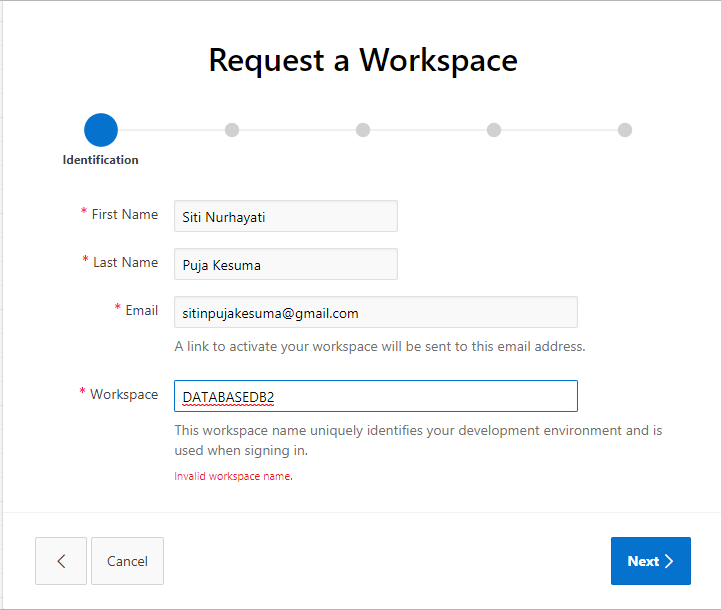
\includegraphics[scale=0.2]{Apex/3.png}
	\centering
	\end{figure}

	\item Mengisi survey seperti dibawah ini 
	\begin{figure} [!htbp]
	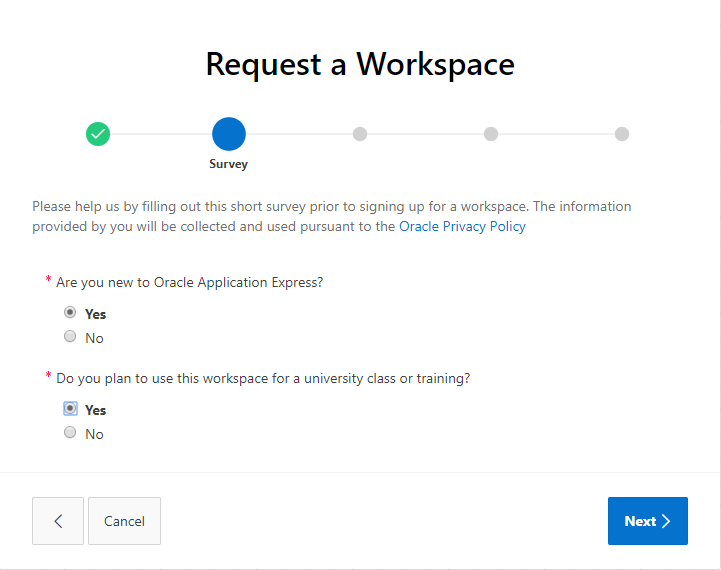
\includegraphics[scale=0.2]{Apex/4.png}
	\centering
	\end{figure}
	
	\item Mengisi Justification
	\begin{figure} [!htbp]
	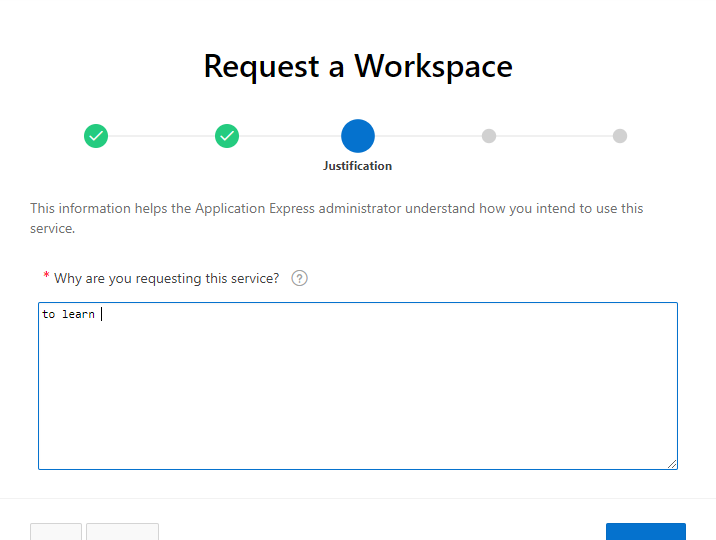
\includegraphics[scale=0.2]{Apex/5.png}
	\centering
	\end{figure}
	
	\item Mencentang Agreement 
	\begin{figure} [!htbp]
	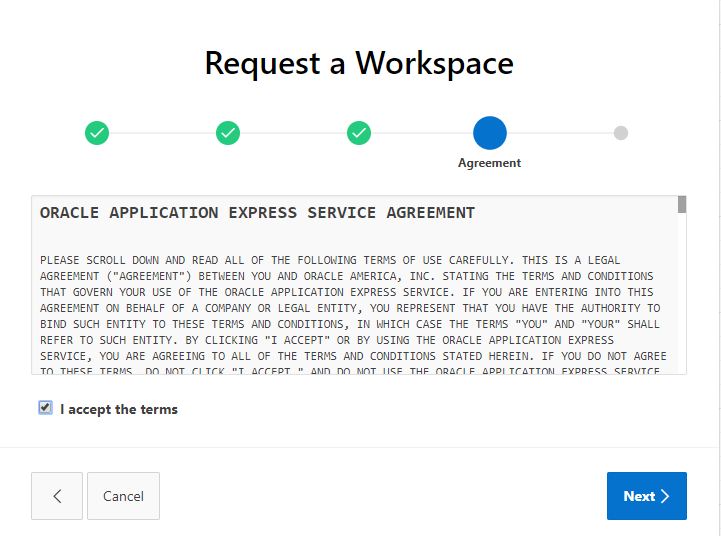
\includegraphics[scale=0.2]{Apex/6.png}
	\centering
	\end{figure}
	
	\item Dan submit Request
	\begin{figure} [!htbp]
	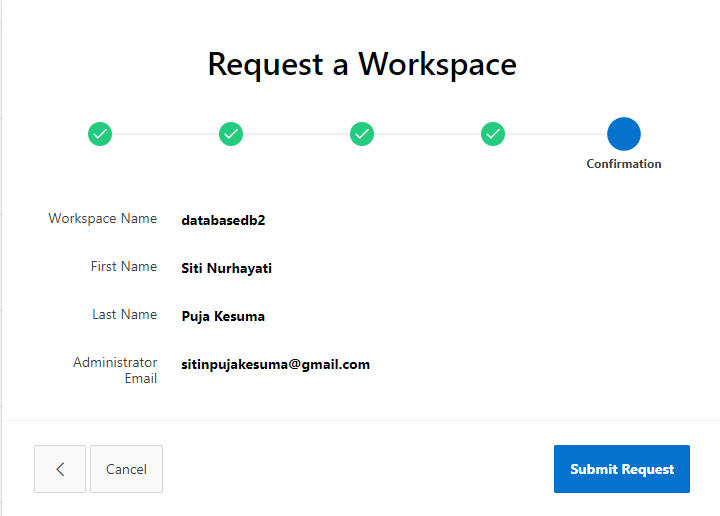
\includegraphics[scale=0.2]{Apex/7.png}
	\centering
	\end{figure}
	
	\item Tunggu email yang akan di kirimkan oleh oracle application seperti dibawah ini 
	\begin{figure} [!htbp]
	
\includegraphics[scale=0.2]{Apex/9.png}
	\centering
	\end{figure}
	
	\item Dan akan mendapatkan email seperti dibawah ini lalu klik create workspaces 
	\begin{figure} [!htbp]
	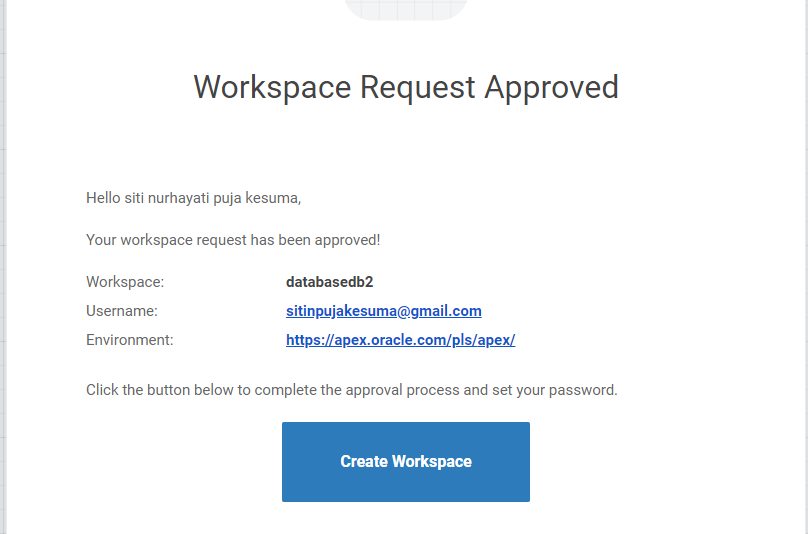
\includegraphics[scale=0.2]{Apex/10.png}
	\centering
	\end{figure}
	
	\item Workspace Succesfully akan muncul seperti gambar dibawah ini dan kllik continue to sign in screen
	\begin{figure} [!htbp]
	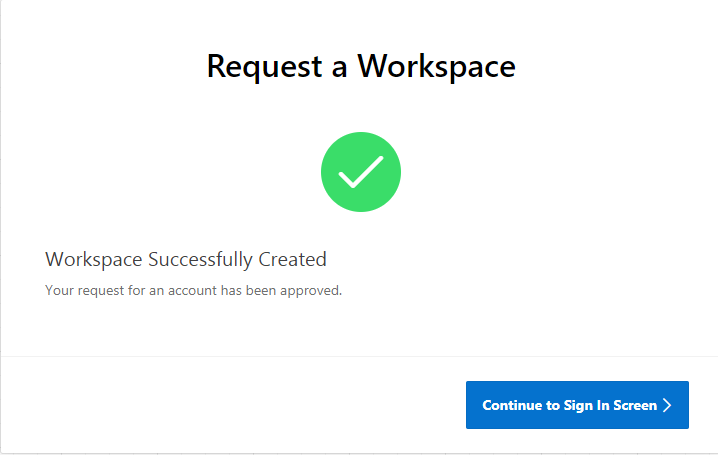
\includegraphics[scale=0.2]{Apex/11.png}
	\centering
	\end{figure}
	
	\item dan pilih App Builder
	\begin{figure} [!htbp]
	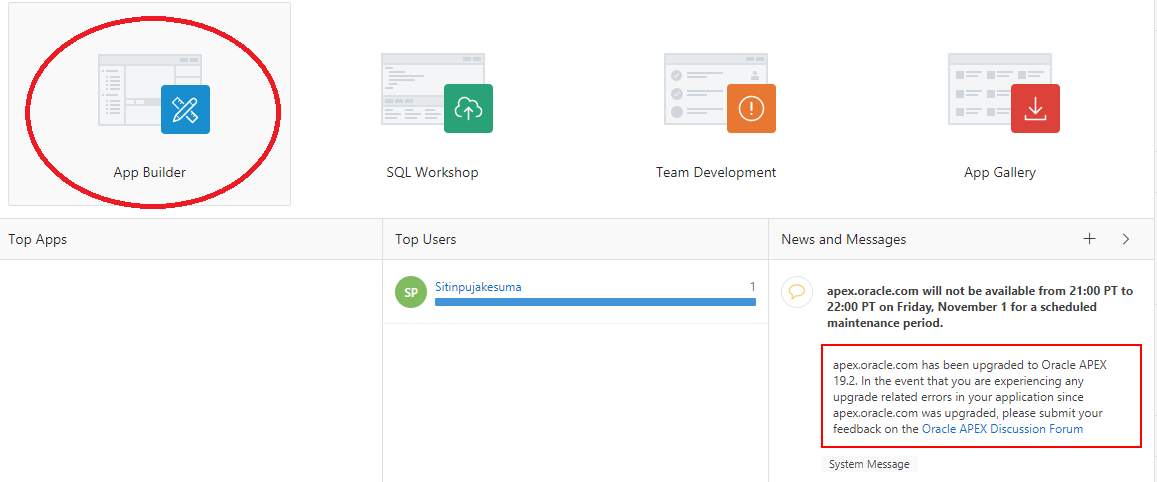
\includegraphics[scale=0.2]{Apex/13.png}
	\centering
	\end{figure}
	
	\item Lalu pilih create yang seperti digambar 
	\begin{figure} [!htbp]
	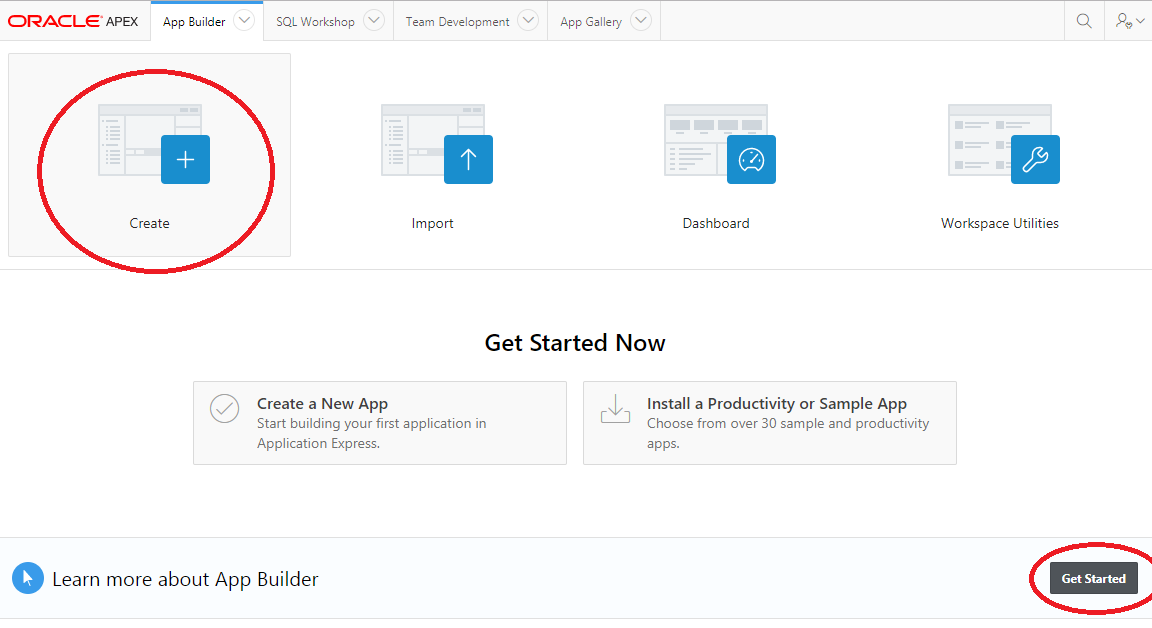
\includegraphics[scale=0.2]{Apex/14.png}
	\centering
	\end{figure}
	
	\item Lalu siapkan file yang akan di import ke exelworkbook atau CSV seperti yang ada digambar 
	\begin{figure} [!htbp]
	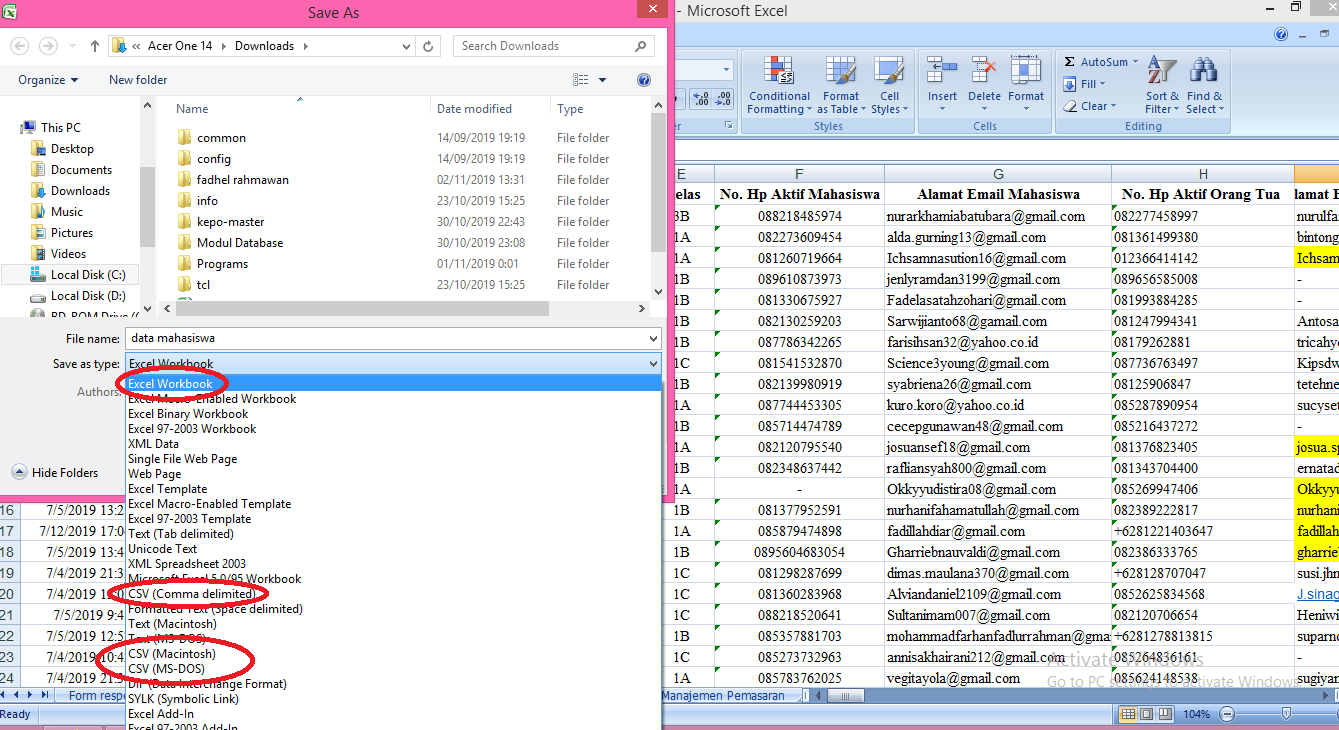
\includegraphics[scale=0.2]{Apex/32.png}
	\centering
	\end{figure}

\item lalu pilih From file 
	\begin{figure} [!htbp]
	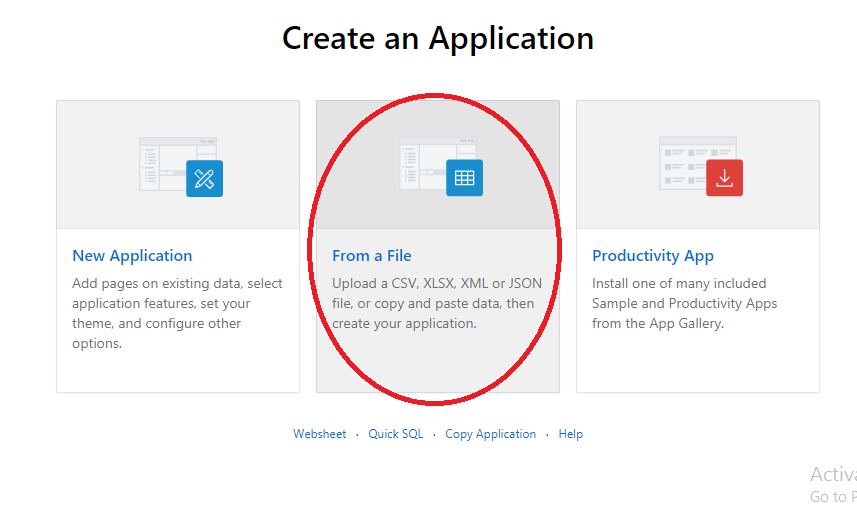
\includegraphics[scale=0.2]{Apex/15.png}
	\centering
	\end{figure}
	
	\item lalu isi form seperti digambar 
	\begin{figure} [!htbp]
	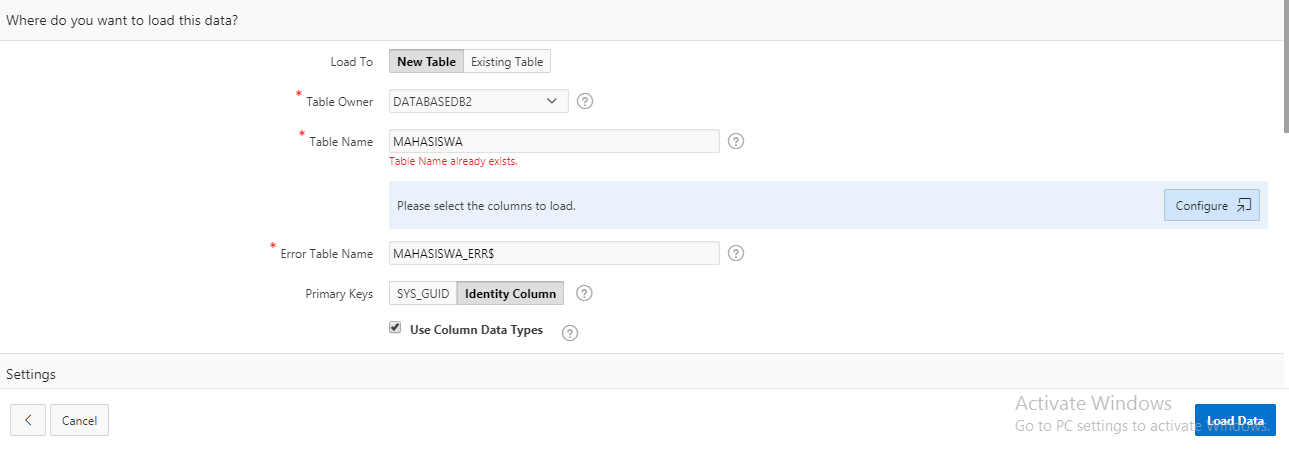
\includegraphics[scale=0.2]{Apex/162.png}
	\centering
	\end{figure}
	
	
	\item Dan akan berhasil seperti dibawah 
	\begin{figure} [!htbp]
	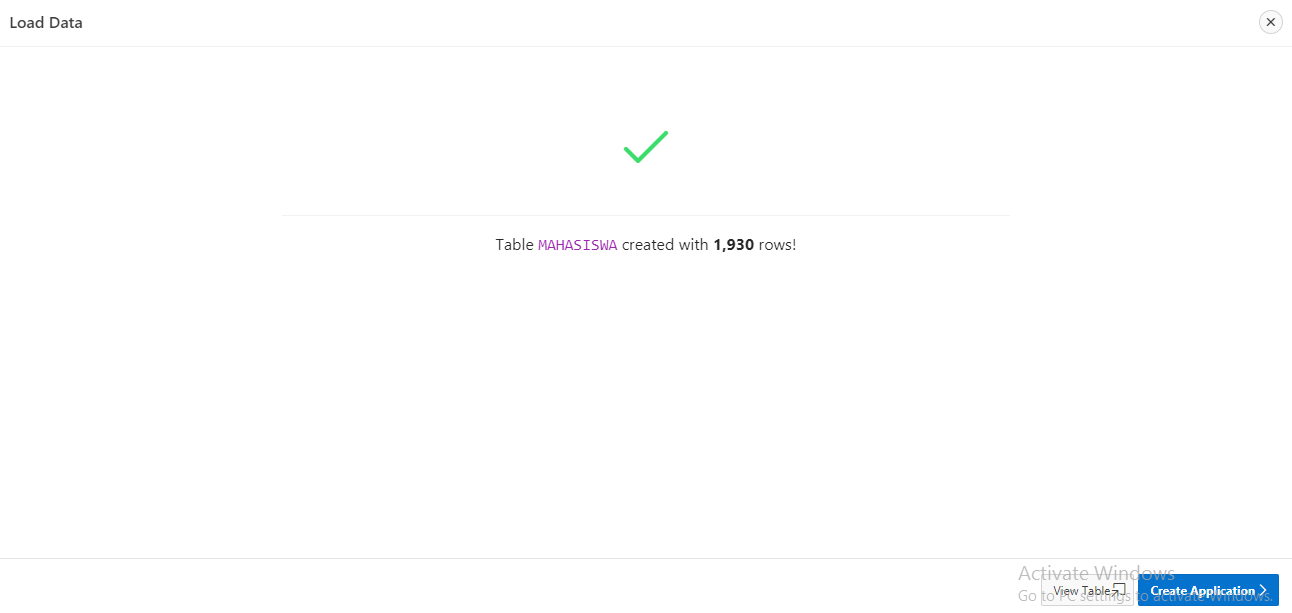
\includegraphics[scale=0.2]{Apex/192.png}
	\centering
	\end{figure}
	
	\item Lalu lanjutkan dengan membuat create aplication
	\begin{figure} [!htbp]
	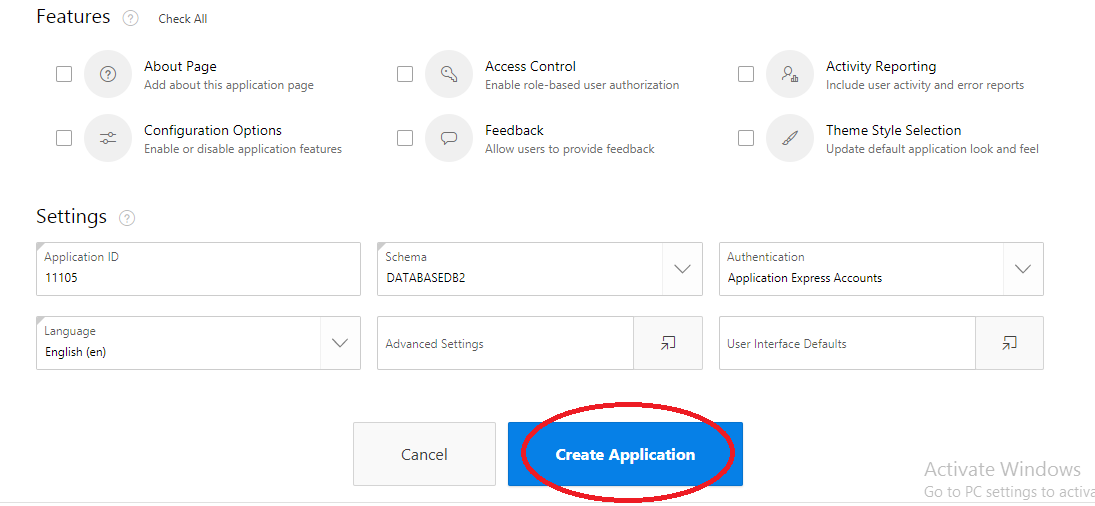
\includegraphics[scale=0.2]{Apex/23.png}
	\centering
	\end{figure}
	\begin{figure} [!htbp]
	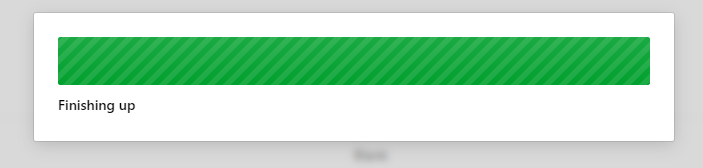
\includegraphics[scale=0.2]{Apex/25.png}
	\centering
	\end{figure}
	
	\item lalu klik run-aplication
	\begin{figure} [!htbp]
	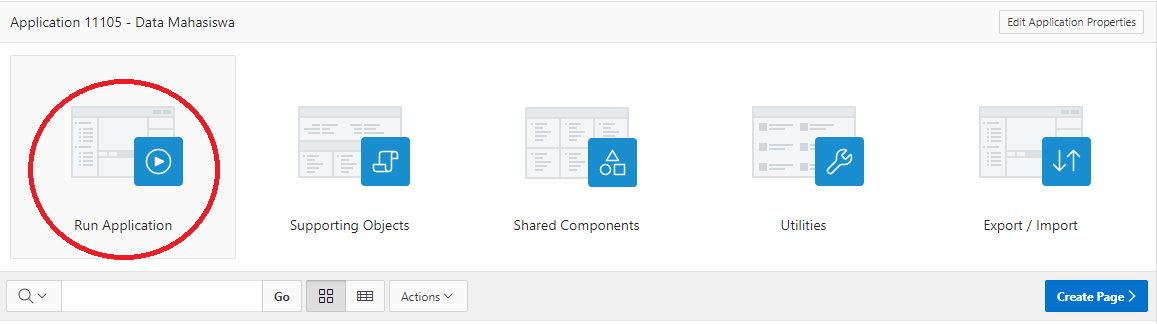
\includegraphics[scale=0.2]{Apex/26.png}
	\centering
	\end{figure}
	
	\item dan login ulang kembali 
	\begin{figure} [!htbp]
	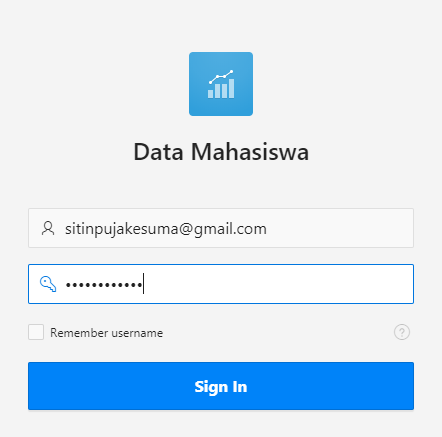
\includegraphics[scale=0.2]{Apex/28.png}
	\centering
	\end{figure}
	
	\item dan akan keluar seperti dibawah ini
	\begin{figure} [!htbp]
	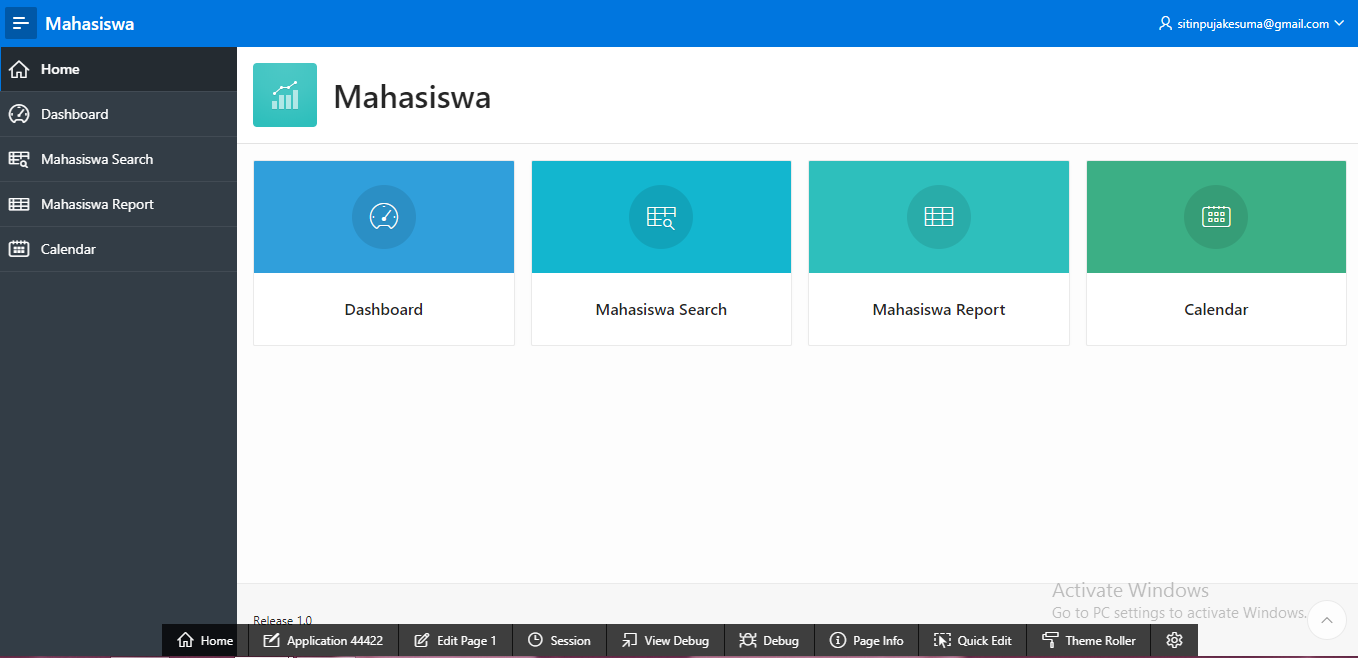
\includegraphics[scale=0.2]{Apex/292.png}
	\centering
	\end{figure}
	
	\item workspace: databasedb2
	password: PUJAKESUMA11
	username: sitinpujakesuma@gmail.com	
	
\end{enumerate}
